\documentclass[examenvragen.tex]{subfiles}

\begin{document}

\section{Newton-Raphson vijfdegraads veelterm}
\subsection{Opgave}
Gegeven een Maple worksheet. (Deze is niet bijgevoegd) Er is een vijfdegraadsveelterm $p(x)$ gegeven met nulpunt $x^* = -0.31$. Er wordt Newton-Rapson gebruikt om dat nulpunt te berekenen en je krijgt een logaritmische plot van de fout. Het plot is een parabool, een typisch plot voor kwadratische convergentie.\\
Verklaar de grafiek van de relatieve fout. Wat is de convergentiesnelheid?
\subsubsection*{Bijvraag}
Het aantal juiste beduidende cijfers verdubbelt bij elke stap. Hoe zie je dat in de grafiek?
\subsection{Informatie}
\begin{itemize}
\item Boek pagina 209: 6 De methode van Newton-Raphson
\item Boek pagina 228: 15 Convergentiesnelheid van rijen
\item Boek pagina 233: Tabel 2.9 Convergentiesnelheden
\end{itemize}
\subsection{Antwoord}
De convergentiesnelheid van Newton-Raphson is gekend.
\begin{itemize}
\item Kwadratisch als $x^*$ een enkelvoudig nulpunt is
\item Lineair als $x^*$ een meervoudig nulpunt is met als convergentiefactor $\rho = 1-\frac{1}{m}$
\end{itemize}
We kunnen aan de grafiek zien welke convergentiesnelheid de methode met het gegeven nulpunt heeft en daaraan zien wat de multipliciteit van het nulpunt $x^{*}$ is.
\begin{figure}[H]
\begin{center}
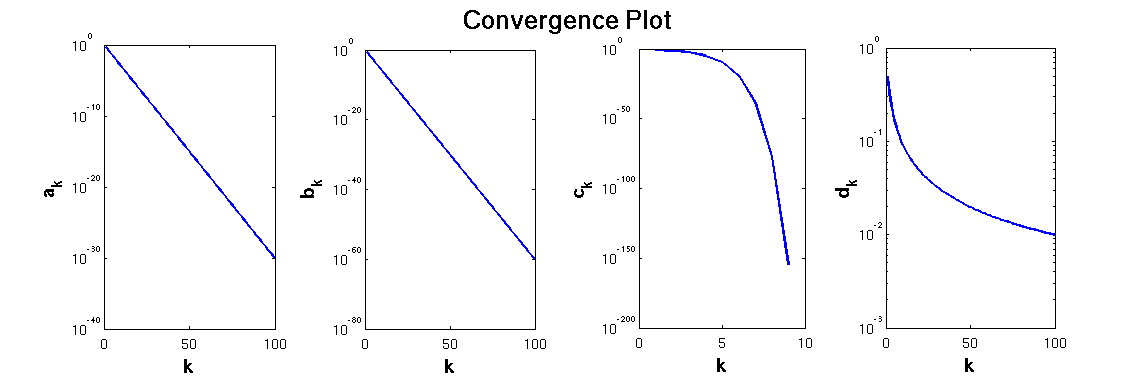
\includegraphics[scale=0.5]{illustraties/vraag_newton_raphson_vijfdegraads_veelterm.png}
\end{center}
\caption{Absolute fout}
\label{fig:vraag_newton_raphson_vijfdegraads_veelterm:abs_err}
\end{figure}
In figuur \ref{fig:vraag_newton_raphson_vijfdegraads_veelterm:abs_err} staan vier plots van absolute fouten. Achtereenvolgens zijn het plots van lineaire, lineaire, quadratische en sublineaire convergentie.
Het aantal juiste beduidende cijfers ver $q$- voudigt in elke iteratiestap, met $q$ gelijk aan de convergentieorde (als de convergentiefactor nul is).

\end{document}
